Alternative splicing is now recognized as a fundamental process in eukaryotic organisms, enabling a single 
gene to generate multiple distinct transcripts. This mechanism affects the majority of human genes 
(\textit{\citep{harrow2006gencode, tress2007implications, kim2008alternative, wang2008alternative, chen2009mechanisms}}) 
and is widely pervasive, playing a crucial role in enhancing the diversity of
the proteome. 
Recent genome-wide studies indicate that 40--60\% of human genes have alternatively spliced forms (\textit{\citep{modrek2002genomic}}). 
This extensive occurrence underscores the need to investigate the evolutionary and conservation patterns of transcript sets, as these 
insights are essential for a deeper understanding of the mechanisms that influence gene evolution.


Understanding the evolution of sets of alternative transcripts is a challenging task and requires automated methods and tools to compare
sets of alternative transcripts from homologous genes. 
Alternative transcripts from homologous genes have traditionally been compared using pairwise spliced 
alignments (PSpAs). A PSpA aligns either a spliced RNA sequence or its DNA equivalent, the coding DNA 
sequence (CDS), with an unspliced DNA sequence. This approach helps identify homologous or corresponding 
exons between sequences, providing crucial insights for genome annotation and gene prediction
(\textit{\citep{stanke2006augustus, dunne2018omgene}}). Various methods have been developed to tackle 
different versions of the PSpA problem, which involves finding the best PSpA between two sequences based 
on a specific optimization function (see \textit{\citep{jammali2019splicedfamalign}}). However, PSpA is limited to 
comparing only two sequences at a time, making it unsuitable for examining the evolution of alternative splicing. 
This restriction also renders it ineffective for analyzing large databases, where multiple sequence comparisons are 
essential.

A logical extension of pairwise spliced alignment (PSpA) for studying the evolution of alternative spliced RNA sets is 
multiple spliced alignment (MSpA). This approach aligns a collection of spliced RNA sequences with their corresponding 
unspliced genomic sequences, allowing for detailed analysis of splicing and exon structures within the gene sequences. 
Unlike traditional multiple sequence alignment (MSA), which focuses solely on sequence similarity, MSpA incorporates the 
splicing and exonic architectures of the input genes. Just as MSA has greatly advanced our understanding of sequence 
evolution, MSpA is anticipated to reveal new insights into the evolution of alternative splicing and the relationships 
among alternative spliced RNA sets.

The MSpA framework also has practical applications for genome annotation by facilitating the identification of exons homologous 
to those in well-characterized species, thereby aiding in the prediction of conserved isoforms in newly annotated genomes.

In the current state of art, there are a few methods available for coomputong MSpAs, with SplicedFamAlignMulti (SFAM) being a 
leading approach (\textit{\citep{jammali2022pairwise}}). SFAM include three extensions : SFAM\_mblock, SFAM\_tcoffee\_p, 
and SFAM\_tcoffee\_m, each providing tailored functionalities for different alignment scenarios. A summary of SFAM methods 
mechanisms is shown in Figure~\ref{fig:spfam-ov}.

\begin{figure}
    \centering
    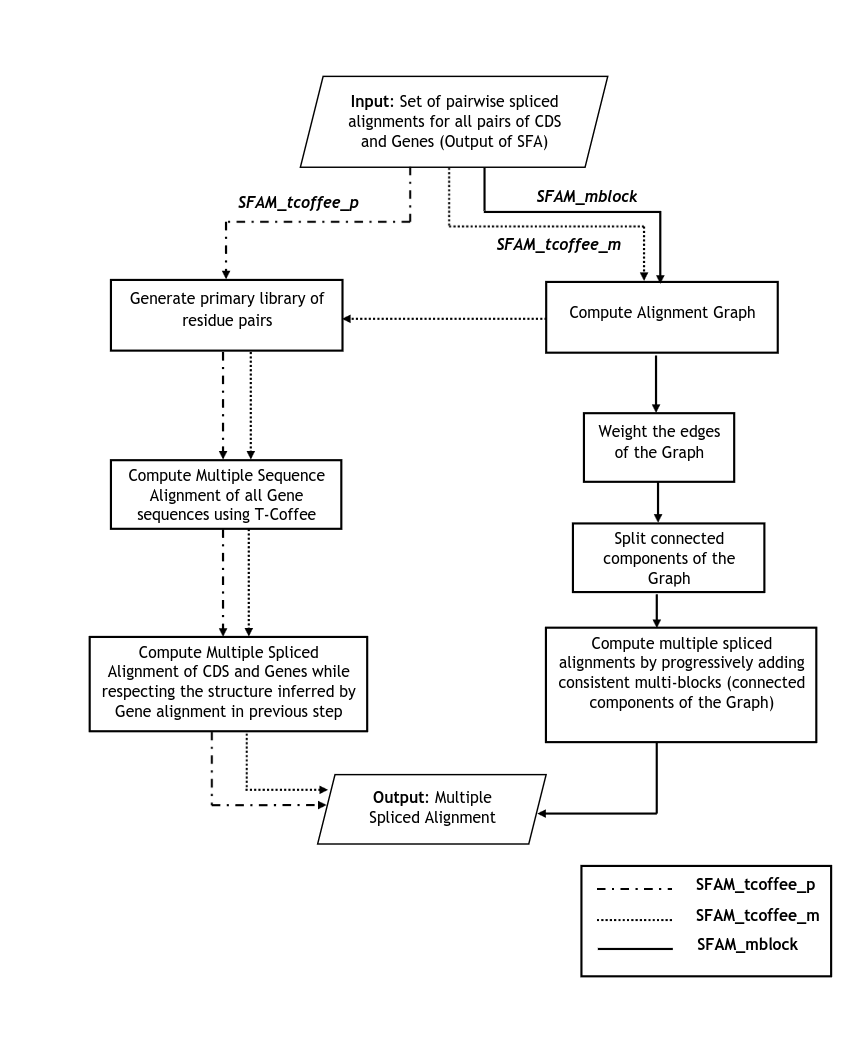
\includegraphics[width=0.3\linewidth]{figures/overview_spFam_methods.png}
    \caption{overview SFAM methods}
    \label{fig:spfam-ov}
\end{figure}

In this report, we present SplicedFamAlignMultiCBA (SFAM\_CBA), a greedy heuristic method developed to merge all 
pairwise spliced alignments (PSpAs) of known coding sequences (CDSs) and gene sequences within a gene family into a 
multiple spliced alignment (MSpA).

